% Chama o arquivo facet-bsi.cls que contém o modelo.
\documentclass{facet-bsi}

% Coloque aqui o nome da Instituição, caso esteja diferente.
\institution{Universidade Federal da Grande Dourados}

% Coloque aqui o nome da faculdade, caso esteja diferente.
\faculty{Faculdade de Ciências Exatas e Tecnologia}

% Coloque aqui o nome do curso.
\course{Bacharelado em Sistemas de Informação}

% Aqui você define o título deste trabalho.
\title{Modelo para escrita de textos de Monografia para o Curso de BSI}

% Aqui você define o nome do seu orientador.
\leader{Rodrigo Porfírio da Silva Sacchi}

% Caso seu trabalho tenha um co-orientador, descomente a primeira linha, coloque o nome do seu orientador
% e comente ou apague a linha com as chaves vazias.

\defcoleader{Co-Orientador: }
% \defcoleader{}
\coleader{Ciclano de Tal}
% \coleader{}

% Coloque aqui o(s) nome(s) do(s) autor(es), separe os nomes com \\ caso tenha mais de um autor.
\author{Matheus de Mattos Pereira \\ Fulano de Tal}

% Aqui você define o mês que será exibido no trabalho, deixe um espaço após o mês.
\mes{Junho }

% Aqui você define o ano que será exibido no trabalho.
\ano{2014}

% Aqui você define o dia da sua apresentação do TCC.
\dia{20 }
% Para a versão final de seu TCC é necessário inserir os dois membros que irão fazer parte da banca 
% avaliadora. Caso esteja fazendo a versão final de seu TCC, insira o nome dos membros da banca, ou senão, 
% deixe os comandos seguintes com chaves vazias. {}
\firstmember{Profª. Drª Bruxa do 71}
\secondmember{Prof. Dr. Seu Madruga}


\begin{document}
  % Diz que o documento deve começar na página 1 e em algarismos romanos.
  \setcounter{page}{1}
  \pagenumbering{roman}
   
  % Com esse comando você cria a capa do trabalho.
  \maketitle

  % Com esse comando você cria a folha de rosto do trabalho.
  \folhaderosto
    
  % Para a versão final de seu TCC, precisa imprimir uma folha de aprovação.
  % Descomente a linha abaixo para criar a folha de aprovação.
  \folhadeaprovacao
  
%   \fichacatalografica
  
  % Define o espaçamento entre as linhas, não comente.
  \onehalfspacing

  % Para a versão final de seu TCC, é possível colocar agradecimentos a pessoas que te ajudaram. É 
  % importante colocar um agradecimento pelo menos para o orientador. 
  \chapter*{Agradecimentos} \thispagestyle{empty}

Agradeço minha família, meu orientador, meu cachorro ...
 
% Aconselhavel que coloque um agradecimento, pelo menos para o orientador.
  
  % Através dessa seção você pode inserir seu resumo do trabalho.
  \chapter*{Resumo} \thispagestyle{empty}

O resumo deverá descrever todo o trabalho, incluindo objetivos, justificativas, metodologia, resultados 
obtidos e conclusões. Não deverá ter mais do que 250 palavras e deverá ser escrito na forma de um único 
parágrafo. O resumo deve ser feito por último.


\smallskip
\noindent \textbf {Palavras-chave: } {LaTeX. Rock. Modelo de TCC. } % Dentro da última chave deve ser 
% inserida as palavras-chaves do trabalho.

  % Essa linha controla as configurações do estilo dos capítulos, não é necessário alterar.
  \estilodapagina
  
  % Essa linha cria o sumário do trabalho.
  \tableofcontents \thispagestyle{empty}
  
  % Os comandos \setcounter e \pagenumbering{} servem para definir a númeração de páginas como 
  % arábica a partir da primeira página do primeiro capítulo. Portanto, não alterem essas duas 
  % linhas seguintes 
  
  
  % Abra o arquivo introducao.tex para editar o primeiro capítulo do texto.
  
  \chapter{Introdução}

% Comando dizer que essa é a primeira página.
\setcounter{page}{1}
\pagenumbering{arabic}

O rock, nascido no século XX e sendo até hoje um dos gêneros mais influentes da música, é um dos 
ritmos musicais mais conhecidos do mundo até hoje. Seja expressando problemas sociais que afetam a 
sociedade através de guitarras e amplificadores, ou ainda criando riff's marcantes que são 
lembrados até hoje, o rock se tornou mais do que um gênero musical. Se tornou uma forma de 
expressão para os artistas de sua época, que são lembrados geração após geração até os dias de hoje.

Oriundo do blues, resultado da fusão entre a música negra e européia, o rock surgiu logo após a 
Segunda Guerra Mundial, aonde uma chamada ``geração silenciosa''se viu a frente de um ritmo 
marginalizado, e desconhecido até então.
 
% A introdução deve indicar o assunto, o problema abordado, a justificativa/motivação e
% os objetivos do trabalho. Pode incluir uma sucinta descrição da metodologia que será usada 
% para resolver um problema, quando for o caso. Deve também indicar o conteúdo de cada 
% capítulo. 

% A introdução deve responder as seguintes perguntas: Qual é o assunto ou problema 
% abordado no trabalho? Por que esse assunto ou problema está sendo abordado? O que deseja-
% se obter com o trabalho? Como pretende-se chegar aos objetivos. A introdução deve ser 
% revisada quando a escrita de todo o TCC estiver concluída._
  
  % A partir deste ponto você pode inserir e/ou retirar capítulos do texto conforme a demanda, com
  % exceção dos capítulos de conclusão e referências bibliográficas.
  \chapter{A história do Rock'n roll}

\section{A Origem negra}


A origem de um estilo musical difundido por todos os cantos do planeta não 
haveria de ter uma 
explicação fácil, afinal, foi longo o caminho necessário para que o rock pudesse nascer.

Diversos ritmos e comportamentos foram se adaptando com o tempo e, em uma pura combinação de 
fatores, surgiu primeiro o {\it rhythm and blues} e depois o {\it rock and roll} propriamente 
dito. Uma retrospectiva pelas raízes é necessária para que se possa entender sua importância no 
cenário, não apenas musical, mas também social do mundo.

O {\it rhythm and blues} é a vertente negra do Rock. É ali que vamos buscar, quase que exclusivamente 
as origens corpóreas do Rock. Reprimidos pela sociedade wasp ({\it white, anglo-saxon and protestant}), 
a mão-de-obra negra, desde os tempos da escravidão, se refugiava na música (os {\it blues}) e na dança 
para dar vazão, pelo corpo, ao protesto que as vias convencionais não permitiam. \cite{CHA1985}

Em suas origens, o rock and roll era essencialmente uma música afro-americana. Os ritmos 
sincronizados, a voz rouca e sentimental e as vocalizações de chamado-e-resposta características dos 
trabalhadores negros eram parte da herança da música africana e tornaram-se tijolos com os quais o 
{\it rock and roll} foi construído. \cite{FRI1996}.

\section{Um pitada de folk e country}

Embora, grande parte da população branca dos Estados Unidos não aceitasse a música dançante dos 
negros, o {\it rythim e blues} ia conquistando admiradores. Não apenas os negros poderiam extravasar suas 
angústias e 
tristezas se divertindo com o novo e frenético som. Agora, os brancos queriam participar e também 
fizeram sua contribuição para o nascimento do {\it rock and roll}.

As músicas {\it folk} e {\it country} dos brancos criavam baladas sobre o cotidiano de pessoas comuns. 
Assim 
como o {\it rhythm and blues} negro, que até esse momento não se misturava, a música {\it country} branca 
também 
buscava 
manifestar suas experiências e emoções e representava uma alternativa às canções melosas e rimadas 
das músicas populares da época.

Assim como a música transmitia a emoção do artista, o público respondia, na mesma medida, movendo 
seus corpos em vibrações que acompanhavam o movimento dos artistas \cite{FRI1996} O 
{\it rock and roll} era, para muitos, um catalisador de identidade para os adolescentes que, criados por 
pais hierarquicamente influenciados pela estrutura do exército, do trabalho e da família, não 
queriam obedecer a regras apenas porque elas existiam. Queriam seguir o rumo que suas próprias vidas 
os levariam.

Apenas alguns anos após o término da II Guerra Mundial, a juventude americana, ainda traumatizada 
pelas perdas humanas — principalmente de jovens –, queria, após anos de sofrimento, se divertir. 
Músicas despretensiosas, ritmos dançantes e o clima de festa serviriam para alegrar tanto os 
músicos, quanto os ouvintes.

Nesse contexto, ocorreu a mistura de música branca e negra que, mais alguns anos depois, já na 
década de 1960, percebendo que já viviam miscigenados através do {\it rock and roll}, vão reclamar e 
protestar contra o racismo.
Foi dessa forma, por meio da festa e da diversão, que brancos e negros aprenderam a dançar e cantar 
juntos.

\section {O rockabilly pede licença: finalmente a mistura se completa}

O {\it rhythm and blues}, originado do {\it blues} (rural e urbano), da música gospel e do {\it jump band 
jazz}, surgiu para 
os 
negros, popularizou-se e espalhou-se.
O {\it folk} e o {\it country} dos brancos se modernizaram e passaram a ser tocados nas rádios. Aos poucos, 
quase que imperceptivelmente, os dois caminhos começaram a se aproximar e, alguns jovens, ansiosos 
por sair da monótona música
popular americana, decidiram criar uma nova estrutura de som e ritmo.

“Em meados do anos 50, alguns jovens, influenciados por Williams, ansiavam por mais. Cientes da 
força e da emocionalidade do {\it rhythm and blues}, eles quiseram incorporar ‘a batida’ à autêntica 
música country. Elvis Presley – nascido no Mississipi e depois estabelecido em Memphis – entrou na 
gravadora {\it Sun Records} em uma tarde de julho para gravar um {\it blues} rural intitulado {\it That’s 
All 
Right 
(Mama)}.

Gravado com apenas um violão, uma guitarra, um baixo e cantado com trêmulo e displicente abandono, 
Elvis criou a síntese do {\it country/blues/rhythm and blues} conhecida como {\it rockabilly}. Mais tarde, 
a 
bateria 
somou-se 
ao conjunto e o {\it rockabilly} tornou-se um gênero de transição para alguns artistas brancos, atraindo 
astros como Jerry Lee Lewis, Johnny Cash, Carl Perkins e Roy Orbinson para a {\it Sun Records} antes do 
final da década”.
% \subsection{Início dos anos 1950 e 1960}
% 
% \subsubsection{Rock and Roll}
% O rock and roll surgiu nos subúrbios dos Estados Unidos no final dos anos 1940 e início da década de 1950 e rapidamente se espalhou para o resto do mundo.
% No começo, o novo estilo rock sofreu várias críticas negativas e algumas positivas, mas sempre atrapalhando seus trabalhos. Muitos diziam que o "novo" rock 
% incentivava o satanismo. Suas origens imediatas remontam a uma mistura entre blues e country, mas com influência de vários gêneros musicais com o rhythm and
% blues.3 . Em 1951, na cidade de Cleveland (no Estado do Ohio), o discotecário Alan Freed começou a tocar a mistura de blues, country e rhythm and blues para 
% uma plateia multirracial e a ele é creditado a primeira utilização da expressão "rock and roll" para 
% descrever a música \cite{friedlander1996rock}. % arrumar
% 
% 
% \subsection{Era de Ouro}
% 
% No Reino Unido, o movimento trad jazz levou muitos artistas do blues a visitar o país. Enquanto estava desenvolvendo o Concorde,
% o sucesso "Rock Island Line", de Lonnie Donegan, em 1955, foi a principal influência e ajudou a desenvolver uma nova tendência de 
% grupos musicais de skiffle em todo a Grã-Bretanha, incluindo os Beatles. Foi em solo britânico que se desenvolveu uma grande cena rock and roll, 
% sem as barreiras raciais que mantiveram a "gravações de raça" ou rhythm and blues separados nos 
% Estados Unidos\cite{castro2008web}. % arrumar
% 
% \section{Os melhores álbuns de rock de todos os tempos}
% 
% De acordo com ..., esses são os melhores álbuns da música.
% %\flushleft
% \begin{table}[!htb]
%   \centering
%   \caption{Titulo da tabela aqui.}
% \begin{tabular}{|c|c|c|c|}
% \hline
% \textbf{Posição} & \textbf{Nome do Album} & \textbf {Nome da banda} & \textbf {Ano} \\
% \hline
% 1 & Sgt. Pepper's Lonely Hearts Club Band & The Beatles & 1967 \\
% \hline
% 2 & Dark Side of the Moon & Pink Floyd & 1973 \\
% \hline
% 3 & Thriller & Michael Jackson & 1982 \\
% \hline
% 4 & Led Zeppelin IV & Led Zeppelin & 1982 \\
% \hline
% 5 & The Joshua Tree & U2 & 1987 \\
% \hline
% 6 & Exile on Main St. & The Rolling Stones & 1972 \\
% \hline
% 7 & Tapestry & Carole King & 1970 \\
% \hline
% 8 & Highway 61 Revisited & Bob Dylan & 1965 \\
% \hline
% 9 & Pet Sounds & The Beach Boys & 1966 \\
% \hline
% 10 & Revolver & The Beatles & 1966 \\
% \hline
% 11 & Ten & Pearl Jam & 1991 \\
% \hline
% 12 & Abbey Road & The Beatles & 1969 \\
% \hline
% 13 & Supernatural & Santana & 1999 \\
% \hline
% 14 & Metallica & Metallica & 1991 \\
% \hline
% 15 & Born to Run & Bruce Springsteen & 1975 \\
% \hline
% 16 & Music from the Motion Picture ``Purple Rain'' & Prince & 1984 \\
% \hline
% 17 & Back in Black & AC/DC & 1980 \\
% \hline
% 18 & Let it Bleed & The Rolling Stones & 1969 \\
% \hline
% 19 & The Doors & The Doors & 1967 \\
% \hline
% 20 & America Beauty & Grateful Dead & 1970 \\
% \hline
% 21 & Come on Over & Shania Twain & 1997 \\
% \hline
% 22 & Who's Next & The Who & 1971 \\
% \hline 
% 23 & Songs in the Key of Life & Stevie Wonder & 1976 \\
% \hline
% 24 & Rumours & Fletwood Mac & 1977 \\
% \hline
% 25 & The Wall & Pink Floyd & 1979 \\
% \hline
% 26 & Jagged Little Pill & Alanis Morissette & 1995 \\
% \hline 
% 27 & Come Away with Me & Norah Jones & 2002 \\
% \hline
% 28 & The Marshall Mathers LP & Eminem & 2000 \\
% \hline
% 29 & Speakerboxx/The Love Below & OutKast & 2003 \\
% \hline
% 30 & The Chronic & Dr. Dre & 1992 \\
% \hline
% 31 & Licensed do Ill & Beastie Boys & 1986 \\
% \hline
% 32 & Appetite for Destruction & Guns N' Roses & 1987 \\
% \hline
% 33 & Wide Open Spaces & Dixie Chicks & 1998 \\
% \hline
% 34 & Kind of Blue & Miles Davis & 1959 \\
% \hline
% 35 & Hotel California & Eagles & 1976 \\ 
% \hline
% 36 & Hysteria & Def Leppard & 1987 \\
% \hline 
% 37 & Grease & Vários artistas & 1977 \\
% \hline
% 38 & What's Going On & Marvin Gaye & 1971 \\
% \hline
% 39 & White Album & The Beatles & 1968 \\
% \hline
% 40 & Saturday Night Fever & Vários artistas & 1977 \\
% \hline
% % 41 & Are You Experienced & Jimi Hendrix & 1967 \\
% % \hline
% % 42 & Revolver & The Beatles & 1966 \\
% % \hline
% % 43 & Boston & Boston & 1976 \\
% % \hline 
% % 44 & Slippery When Wet & Bon Jovi & 1986 \\
% % \hline
% % 45 & Achtung Baby & U2 & 1991 \\
% % \hline
% % 46 & Whitney Houston & Whistney Houston & 1985 \\
% % \hline
% % 47 & Led Zeppelin II & Led Zeppelin & 1969 \\
% % \hline
% % 48 & Crash & Dave Matthews Band & 1996 \\
% % \hline
% % 49 & Sticky Fingers & The Rolling Stones & 1971 \\
% % \hline
% % 50 & Dookie & Green Day & 1994 \\
% 
% \end{tabular}
% \end{table}
  
\chapter{Uma revolução}

\section{O rei do rock'n roll}

% Exemplo de imagem.
\begin{figure}[!htb]
  \centering
  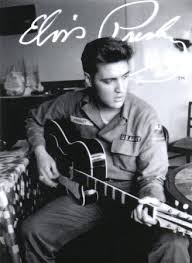
\includegraphics[scale=0.45]{imagens/elvis}
  \caption{Elvis Presley no início de sua carreira.}
  \label{fig:elvis}
\end{figure}

Um dos artistas mais importantes dos primeiros anos do {\it rock’n’roll} foi Elvis Presley. Como explica 
Chacon \cite{CHA1985}, ``só um símbolo sexual, devidamente municiado pelos melhores autores e ‘cantando e 
suando 
como um 
negro`` poderia transformar aquele modismo numa verdadeira revolução”. A sensualidade presente na voz rouca 
e 
na sua maneira de dançar, que transformaram Elvis numa superestrela do rock, tornou-o um exemplo clássico da 
influência negra sobre a sociedade branca norte-americana \cite{CHA1985}. Além disso, sua história também 
tem pontos em comum com a de outros artistas: vidas atribuladas, 
envolvimento com drogas, relacionamentos desfeitos e um triste fim. Estes foram também alguns dos 
ingredientes das vidas de Jerry Lee Lewis, que teve muitos problemas com bebida e se casou várias vezes ou 
de Buddy Holly, que morreu ainda jovem em um desastre de avião.
  
\section{A Era Beatles}

No início de 1956, John Lennon formou o conjunto {\it The Quarrymen}, que nada mais era do que uma reunião 
informal 
de amigos. O grupo se estabilizaria em 1960, com Paul McCartney e George Harrison como guitarristas, Stu 
Sutcliffe no baixo e o baterista Pete Best.

Neste mesmo ano, The Quarrymen deixa de existir; em seu lugar, surge uma “banda profissional de 
{\it rock’n’roll}, os Beatles. O nome foi uma combinação da palavra beetle (besouro) com uma expressão 
comum à 
época para o rock: música {\it beat}. A referência aos insetos foi uma homenagem ao grupo de Buddy Holly, 
chamado 
{\it Crickets} (grilos).

Em 1962, os Beatles foram tocar em Hamburgo, Alemanha, quando encontraram o baterista Ringo Starr, que 
tocava com os {\it Hurricanes}. Pouco tempo depois, ele substituiria Pete Best.

\subsection{A explosão dos Beatles}

Finalmente em agosto deste mesmo ano, o grupo entraria nos estúdios de {\it Abbey Road} para a gravação 
do 
primeiro compacto da banda, com as músicas {\it P.S. I Love You} e {\it Love me Do}. Nesta época, Stu 
Sutcliffe havia 
deixado os {\it Beatles} e Paul tomou a posição de baixista do grupo.
Com o segundo single, {\it Please Please Me}, os {\it Beatles} alcançaram o topo das paradas britânicas.

Em 1963, apenas um ano depois do primeiro lançamento dos {\it Beatles}, a {\it Beatlemania} eclodiu na 
Inglaterra. 
Brian Epstein e o produtor George Martin, da EMI, decidem partir com a banda para os Estados Unidos, cientes 
da popularidade do grupo. Em 1964, os Beatles conquistam a América com {\it I Want to Hold Your Hand}. A 
apresentação da banda no programa de televisão de Ed Sullivan – o mesmo que tinha lançado Elvis Presley – 
foi a alavanca para que a mídia norte-americana passasse a publicar matérias sobre os {\it Fab Four} (como 
eram 
conhecidos).

\begin{figure}[!htb]
%  \vspace{1cm}
  \centering
  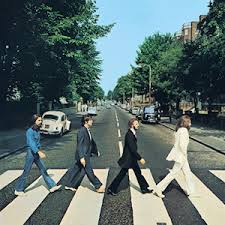
\includegraphics[width=7cm]{imagens/abbey_road}
  \caption{Capa do Album Abbey Road, de 1969.}
  \label{fig:abbeyroad}
%  \vspace{1cm}
\end{figure}

Durante os shows dos {\it Beatles}, quase não se ouvia suas músicas, devido à 
quantidade 
de garotas que gritavam 
histericamente pelos músicos. A partir de 1965, o grupo passou a se preocupar mais com as composições, 
deixando o amor romântico de lado e empenhando-se em explorar outros temas. O disco {\it Rubber Soul}, 
lançado 
neste mesmo ano, marca o amadurecimento da banda, visível na crítica social da música {\it Nowhere Man} ou 
nas 
referências abstratas de {\it Norwegian Wood}, entre outras composições deste disco.


\section{Pedras que rolam}

Entretanto, não só do sucesso dos {\it Beatles} vivia a Inglaterra. {\it Rolling Stones} e {\it The Who} 
são exemplos de 
grupos que surgiram na década de 60 e que marcaram o rock em muitos sentidos.

O verso de uma canção de blues de Muddy Waters – {\it rolling stones gather no moss} (pedras que rolam não 
criam 
musgo) - dá o nome ao conjunto fundado pelo guitarrista Brian Jones. O vocalista, Mick Jagger, torna-se o 
líder da banda após a saída de Jones. A influência negra é uma das marcas do grupo, além da sensualidade e 
uma certa androginia, características da performance de Jagger.

Em 1968, os {\it Stones} exploram o engajamento político na música {\it Street Fighting Man}, influenciados 
pelas 
manifestações políticas de massa que emergiam. A música, composta por Mick Jagger e Keith Richards, torna-se 
hino dos revolucionários e é censurada pela polícia de Chicago.

A música dos {\it Stones} é da mesma época de {\it Revolution}, dos {\it Beatles}. Esta última também foi 
composta a partir do 
contexto político-social de 1968, marcado principalmente pelas manifestações de maio deste mesmo ano. Os 
críticos passam a analisar {\it Revolution} e {\it Street Fighting Man} e a compará-las, sendo que 
consideram a primeira 
como uma “contra-revolução” e a segunda como a “verdadeira revolução”. Mas, tanto as últimas estrofes da 
música dos Stones quanto uma declaração de Jagger – “Eles devem pensar que ‘{\it Street Fighting Man}’ é 
capaz de 
promover uma revolução\ldots Eu bem que gostaria que isso fosse verdade” – demonstram que a idéia dos 
críticos se baseia em suposições.

\section{Melhores riffs da história do rock}

De acordo com a revista The Sun, estes são os 5 melhores riffs da história do rock.

% Exemplo de tabela
\begin{table}[!htb]
  \centering
  \caption{Melhores riffs da história do rock, de acordo com a revista The Sun.}
  \vspace{0.1cm}
\begin{tabular}{|c|c|c|}
\hline
\textbf{Posição} & \textbf{Nome da Música} & \textbf {Nome da banda} \\
\hline
1 & Sweet Child O'Mine & Guns 'N Roses  \\
\hline
2 & Layla & Eric Clapton \\
\hline
3 & Walk This Way & Aerosmith \\
\hline
4 & Beat It & Michael Jackson \\
\hline
5 & Ace of Spades & Motörhead \\
\hline
% 6 & Voodoo Child & Jimi Hendrix \\
% \hline
% 7 & Another One Bites the Dust & Queen \\
% \hline
% 8 & Smell Like Teen Spirit & Nirvana \\
% \hline
% 9 & Smoke on the Water & Deep Purple \\
% \hline
% 10 & American Idiot & Green Day \\
% \hline
\end{tabular}

\end{table}
 
 
  % Abra o arquivo conclusao.tex para editar a conclusão de seu texto.
  \chapter{Conclusão} 

A conclusão deve conter uma recapitulação resumida dos resultados obtidos e indicar
se estes foram suficientes para resolver com eficiência o problema abordado. Pode também
indicar as limitações do sistema desenvolvido e fazer sugestões para trabalhos futuros.

  
  % -------------------------------------------------------------------------------------------
  % Descomente estas duas linhas para inserir o capítulo de referências bibliográficas no texto.
  % Você deve criar um arquivo chamado ourbib.bib, contendo a coleção de sua bibliografia.
  \bibliographystyle{acm}
  \bibliography{ourbib}

\end{document}
